% This LaTeX was auto-generated from MATLAB code.
% To make changes, update the MATLAB code and export to LaTeX again.

\documentclass{article}

\usepackage[utf8]{inputenc}
\usepackage[T1]{fontenc}
\usepackage{lmodern}
\usepackage{graphicx}
\usepackage{color}
\usepackage{hyperref}
\usepackage{amsmath}
\usepackage{amsfonts}
\usepackage{epstopdf}
\usepackage[table]{xcolor}
\usepackage{matlab}

\sloppy
\epstopdfsetup{outdir=./}
\graphicspath{ {./cltExampleBoth_images/} }

\begin{document}

\matlabtitle{How many observations should I make? An application of the central limit theorem to human performance variables }

\begin{par}
\begin{flushleft}
Author: Ross Wilkinson
\end{flushleft}
\end{par}


\matlabheading{Introduction}

\begin{par}
\begin{flushleft}
The central limit theorem states that, under some conditions, the average of many samples (observations) of a random variable with finite mean and variance is itself a random variable – whose distribution converges to a normal distribution as the number of samples increases (Wikipedia).
\end{flushleft}
\end{par}

\begin{par}
\begin{flushleft}
Thus, we can assume that any measure of human performance will follow a normal distribution and that observations will regress toward a finite mean with a standard normal distribution of variance.
\end{flushleft}
\end{par}

\begin{par}
\begin{flushleft}
\textbf{Example}
\end{flushleft}
\end{par}

\begin{par}
\begin{flushleft}
We want to compare the maximal 1-s power output produced by a cyclist during a sprint between two different experimental conditions. But we are unsure of how many observations (number of sprints) we should take under each condition. We also want to know whether sprinting indoors on a traditional stationary ergometer is more or less variable than outdoors. 
\end{flushleft}
\end{par}

\begin{par}
\begin{flushleft}
\textbf{Can we take one sample?}
\end{flushleft}
\end{par}

\begin{par}
\begin{flushleft}
We know that the subject's performance is likely to follow a normal distribution under each condition, so taking one sample (performing one sprint) under each condition has a \textasciitilde{}68\% chance of being within one standard deviation of their true mean and a \textasciitilde{}95\% chance of being within two standard deviations, and a \textasciitilde{}99\% chance of being within three standard deviations. But we have no idea of what the standard deviation is; is it 40 W, 100 W, etc.? and is it more variable on the ergometer or on the bike?
\end{flushleft}
\end{par}

\begin{par}
\begin{flushleft}
\textbf{Can we emprically determine how many observations are sufficient?}
\end{flushleft}
\end{par}

\begin{par}
\begin{flushleft}
The answer is yes. First, we need to verify that the subject's maximal power output follows a normal distribution; we can do this by taking as many observations as feasibly possible. Once we have an approximation of this distribution we can run simulations to test whether taking a certain number of samples is representative of the mean in the long run.
\end{flushleft}
\end{par}

\begin{par}
\begin{flushleft}
\textbf{Can we empirically determine whether testing on the ergo or on the bike is better?}
\end{flushleft}
\end{par}

\begin{par}
\begin{flushleft}
Yes again. One way to do this is to calculate the relative uncertainty of the measurement, which in this case be called the relative intra-individual variability. This is done by taking the root mean square error of all the measurements and dividing by the mean. The threshold for an acceptable level of uncertainty will change depending on the measurement.
\end{flushleft}
\end{par}


\matlabheading{Our experiment}

\begin{par}
\begin{flushleft}
We decide that it is feasible for our subject (Ross) to perform 12 sprints, each seperated by 3 minutes of rest, in one testing session without introducing any dependent variables like fatigue. On day 1, Ross performs 12 sprints on a traditional stationary ergometer. On day 2, Ross performs 12 sprints outside on bike. Once we have our results from each day of testing, we will visualize the data, check for any linear trends, fit a distribution, run some simulations to decide on the number of observations we should take, then compare the level of uncertainty between the ergometer and the bike.
\end{flushleft}
\end{par}


\matlabheading{Our results}

\begin{par}
\begin{flushleft}
Here are the results from each day of 12 sprints in Watts.
\end{flushleft}
\end{par}

\begin{matlabcode}
maxPowerErgo = [1545; 1526; 1526; 1565; 1614; 1544;...
1553; 1611; 1519; 1608; 1571; 1566];

maxPowerBike = [1179; 1145; 1203; 1205; 1201; 1201; 1181;...
    1172; 1221; 1163; 1211; 1171];
\end{matlabcode}


\matlabheading{Visualize the data}

\begin{par}
\begin{flushleft}
\textbf{Histogram}
\end{flushleft}
\end{par}

\begin{par}
\begin{flushleft}
A histogram provides a quick visual insight into how a data set is distributed. The range of possible values is divided into intervals, or \textit{bins}. Then a bar chart is created, where the height of each bar corresponds to how frequently values in that bin appear in the data.
\end{flushleft}
\end{par}

\begin{par}
\begin{flushleft}
Create a histogram of the results seperated into 3 bins.
\end{flushleft}
\end{par}

\begin{matlabcode}
histogram(maxPowerErgo,3)
hold on
histogram(maxPowerBike,3)
hold off
xlabel('Maximal 1-s power output (W)')
ylabel('Number of observations within bin')
legend('Ergo','Bike')
\end{matlabcode}
\begin{center}
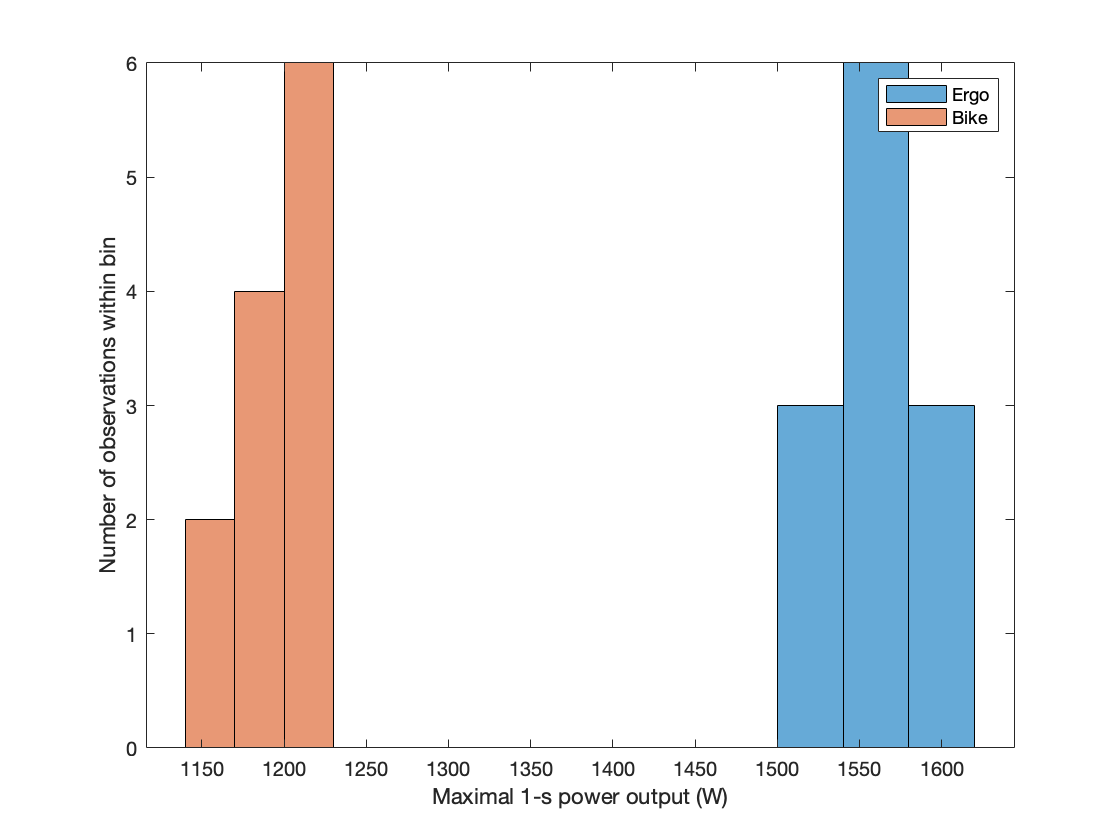
\includegraphics[width=\maxwidth{56.196688409433015em}]{figure_0.png}
\end{center}


\begin{par}
\begin{flushleft}
\textbf{Scatter plots}
\end{flushleft}
\end{par}

\begin{par}
\begin{flushleft}
A scatter plot explores how two variables are related to each other. In this case how maximal power output is related to the trial number.
\end{flushleft}
\end{par}

\begin{par}
\begin{flushleft}
Create a scatter plot of the results across trials 1 to 12.
\end{flushleft}
\end{par}

\begin{matlabcode}
scatter(1:12,maxPowerErgo)
hold on
scatter(1:12,maxPowerBike)
hold off
xlabel('Trial number')
ylabel('Maximal 1-s power output (W)')
legend('Ergo','Bike')
\end{matlabcode}
\begin{center}
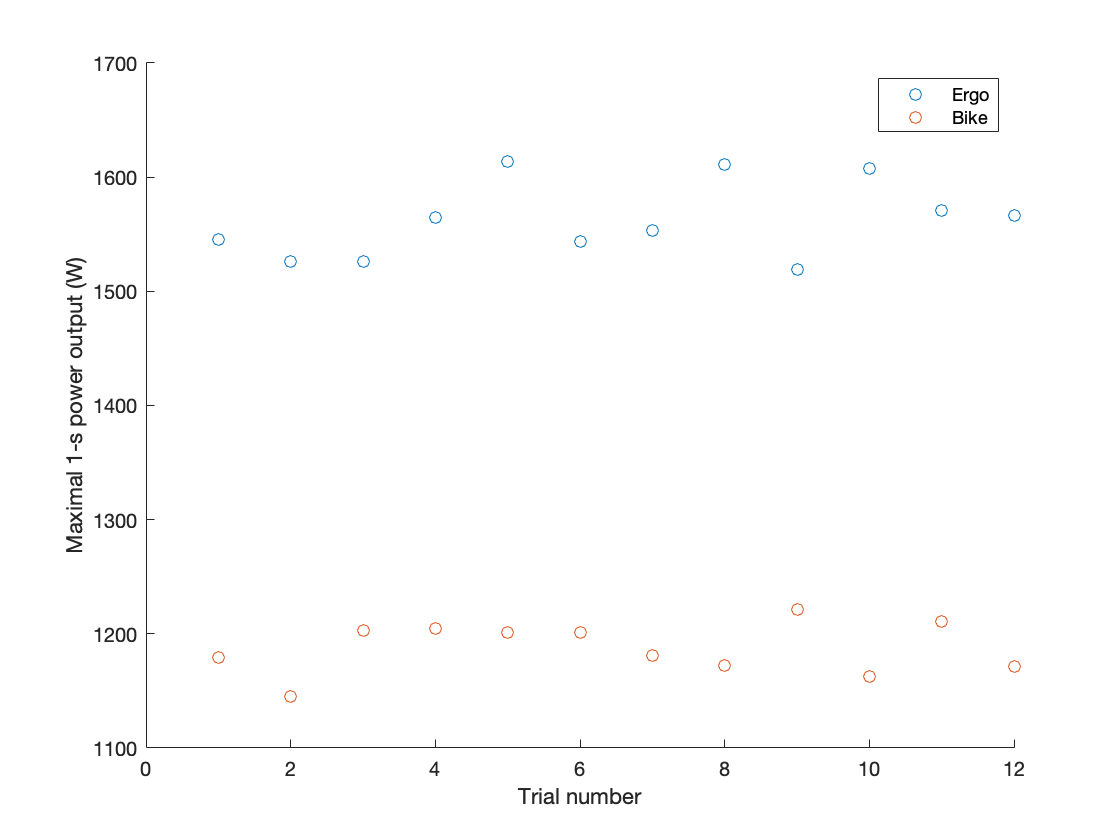
\includegraphics[width=\maxwidth{56.196688409433015em}]{figure_1.png}
\end{center}


\begin{par}
\begin{flushleft}
\textbf{Box plots}
\end{flushleft}
\end{par}

\begin{par}
\begin{flushleft}
A box plot is another way to visualize the distribution of a data set. The central box represents the middle 50\% of observations, with the red line at the median. The "whisker" lines show the extent of \textasciitilde{}99\% of the data. Remaining outliers are shown individually with red crosses. 
\end{flushleft}
\end{par}

\begin{par}
\begin{flushleft}
Create a box plot of the results.
\end{flushleft}
\end{par}

\begin{matlabcode}
boxplot([maxPowerErgo, maxPowerBike])
ylabel('Maximal 1-s power output (W)')
\end{matlabcode}
\begin{center}
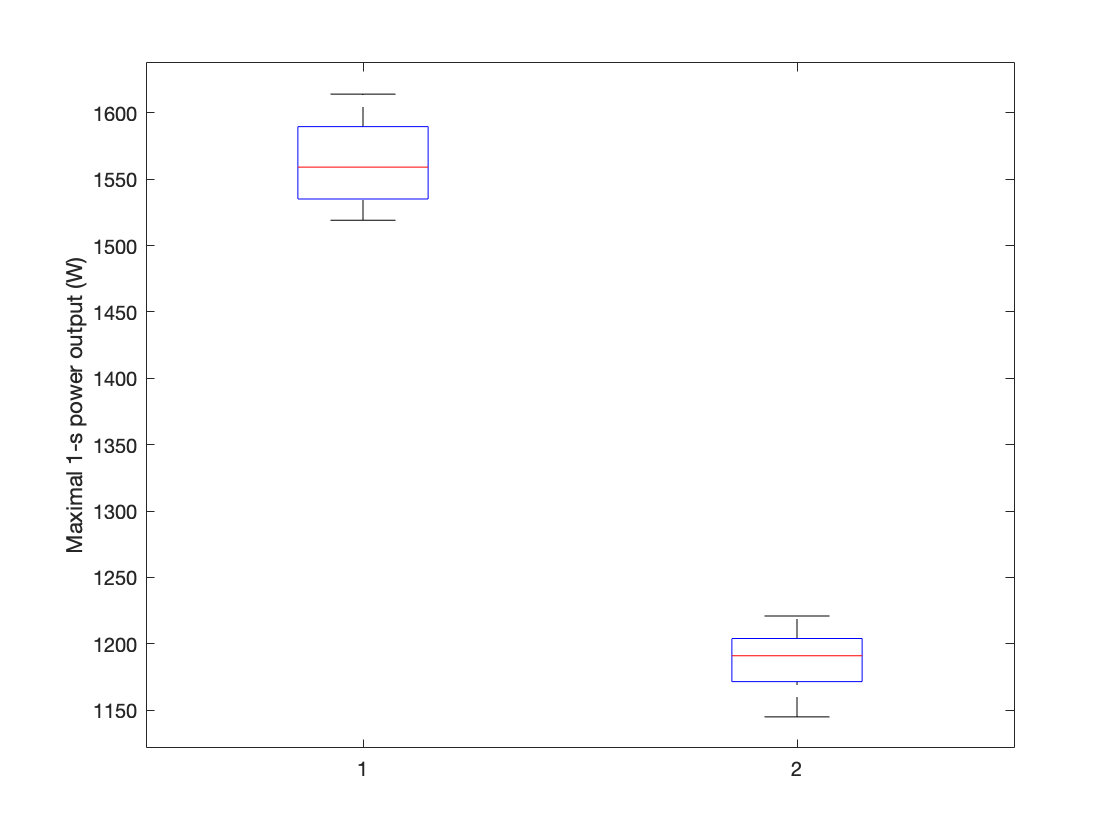
\includegraphics[width=\maxwidth{56.196688409433015em}]{figure_2.png}
\end{center}


\matlabheading{Measures of centrality and spread}

\begin{par}
\begin{flushleft}
Calculate the mean and median of the results
\end{flushleft}
\end{par}

\begin{matlabcode}
meanPwrErgo = mean(maxPowerErgo)
\end{matlabcode}
\begin{matlaboutput}
meanPwrErgo = 1.5623e+03
\end{matlaboutput}
\begin{matlabcode}
medPwrErgo = median(maxPowerErgo)
\end{matlabcode}
\begin{matlaboutput}
medPwrErgo = 1559
\end{matlaboutput}
\begin{matlabcode}
meanPwrBike = mean(maxPowerBike)
\end{matlabcode}
\begin{matlaboutput}
meanPwrBike = 1.1878e+03
\end{matlaboutput}
\begin{matlabcode}
medPwrBike = median(maxPowerBike)
\end{matlabcode}
\begin{matlaboutput}
medPwrBike = 1191
\end{matlaboutput}

\begin{par}
\begin{flushleft}
Calculate the standard deviation (STD) and interquartile range (IQR) of the results
\end{flushleft}
\end{par}

\begin{matlabcode}
stdPwrErgo = std(maxPowerErgo)
\end{matlabcode}
\begin{matlaboutput}
stdPwrErgo = 33.6569
\end{matlaboutput}
\begin{matlabcode}
iqrPwrErgo = iqr(maxPowerErgo)
\end{matlabcode}
\begin{matlaboutput}
iqrPwrErgo = 54.5000
\end{matlaboutput}
\begin{matlabcode}
stdPwrBike = std(maxPowerBike)
\end{matlabcode}
\begin{matlaboutput}
stdPwrBike = 22.5998
\end{matlaboutput}
\begin{matlabcode}
iqrPwrBike = iqr(maxPowerBike)
\end{matlabcode}
\begin{matlaboutput}
iqrPwrBike = 32.5000
\end{matlaboutput}

\begin{par}
\begin{flushleft}
\textasciitilde{}68\% of the results will be within ± one standard deviation from the mean.
\end{flushleft}
\end{par}

\begin{par}
\begin{flushleft}
50\% of the results will be within the IQR from the mean.
\end{flushleft}
\end{par}


\matlabheading{Linear correlation}

\begin{par}
\begin{flushleft}
If we are considering getting our subjects to do less than 12 sprints, then we need to make sure there is no bias as the person performs more sprints.
\end{flushleft}
\end{par}

\begin{par}
\begin{flushleft}
Test whether there is a significant linear correlation between power output and the number of trials at the significance level 0.05. We are interested in the off-diagonal numbers, which correspond to the r-value and p-value.
\end{flushleft}
\end{par}

\begin{matlabcode}
nTrials = 1:12;
[rErgo,pErgo] = corrcoef(nTrials',maxPowerErgo)
\end{matlabcode}
\begin{matlaboutput}
rErgo = 2x2    
    1.0000    0.3671
    0.3671    1.0000

pErgo = 2x2    
    1.0000    0.2405
    0.2405    1.0000

\end{matlaboutput}
\begin{matlabcode}
[rBike,pBike] = corrcoef(nTrials',maxPowerBike)
\end{matlabcode}
\begin{matlaboutput}
rBike = 2x2    
    1.0000    0.1110
    0.1110    1.0000

pbike = 2x2    
    1.0000    0.7313
    0.7313    1.0000

\end{matlaboutput}

\begin{par}
\begin{flushleft}
A p-value \textgreater{}0.05 confirms that no significant linear correlation exists. Suggesting that taking a smaller number of samples will still provide results that are distributed around the mean.
\end{flushleft}
\end{par}


\matlabheading{Data distribution}

\begin{par}
\begin{flushleft}
Fit and plot a normal distribution then compare it to a fitted distribution.
\end{flushleft}
\end{par}

\begin{matlabcode}
xErgo = meanPwrErgo-200:meanPwrErgo+200;
xBike = meanPwrBike-200:meanPwrBike+200;
pdfPwrErgo = normpdf(xErgo,meanPwrErgo,stdPwrErgo);
pdfPwrBike = normpdf(xBike,meanPwrBike,stdPwrBike);
% histogram(maxPowerErgo,3,"Normalization","pdf")
% hold on
% histogram(maxPowerBike,3,"Normalization","pdf")
plot(xErgo,pdfPwrErgo,'linewidth',2)
hold on
\end{matlabcode}

\begin{par}
\begin{flushleft}
Fit a kernel distribution to the data
\end{flushleft}
\end{par}

\begin{matlabcode}
pdErgo = fitdist(maxPowerErgo,'Kernel');
pdBike = fitdist(maxPowerBike,'Kernel');
kerPwrErgo = pdf(pdErgo,xErgo);
kerPwrBike = pdf(pdBike,xBike);
plot(xErgo,kerPwrErgo,'linewidth',2)
plot(xBike,pdfPwrBike,'linewidth',2)
plot(xBike,kerPwrBike,'linewidth',2)
hold off
legend('Normal dist. Ergo','Kernel dist. Ergo','Normal dist. Bike','Kernel dist. Bike')
\end{matlabcode}
\begin{center}
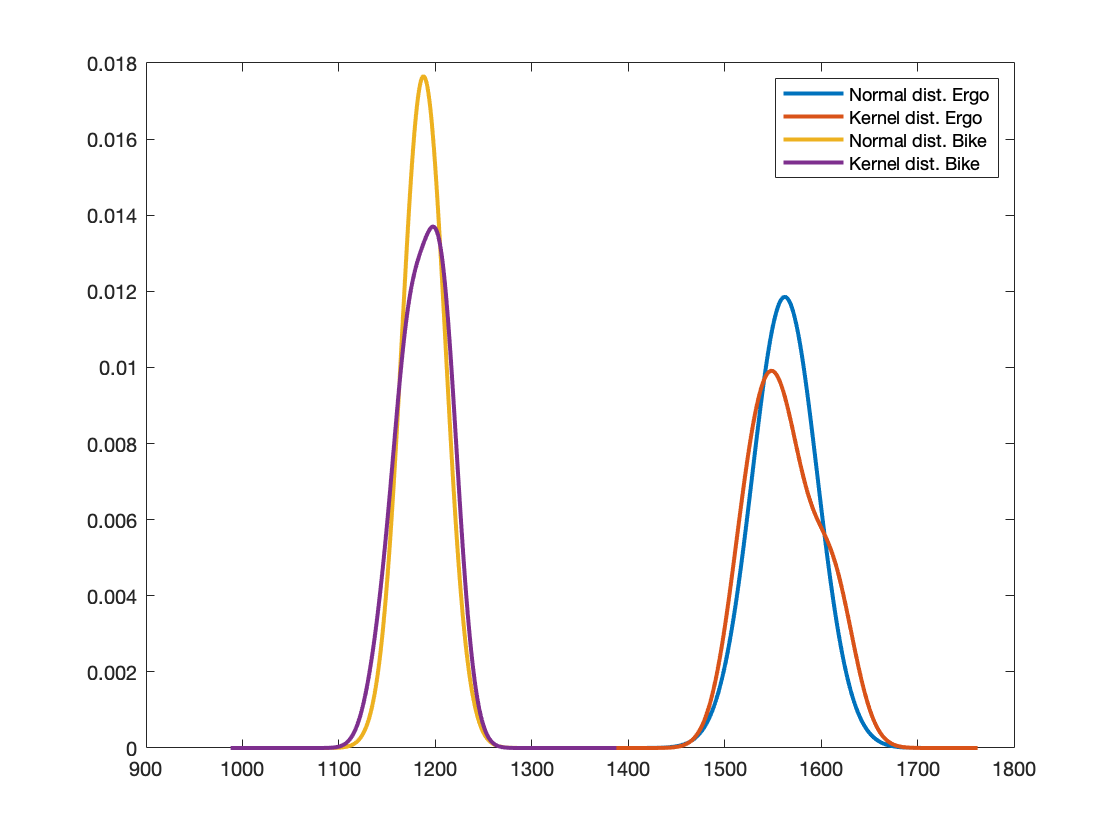
\includegraphics[width=\maxwidth{56.196688409433015em}]{figure_3.png}
\end{center}

\begin{par}
\begin{flushleft}
Test if the results are significantly different from a standard normal distribution. h = 0 confirms the null.
\end{flushleft}
\end{par}

\begin{matlabcode}
zErgo = zscore(maxPowerErgo);
zBike = zscore(maxPowerBike);
[hErgo,pErgo] = kstest(zErgo)
\end{matlabcode}
\begin{matlaboutput}
hErgo = 
   0

pErgo = 0.8595
\end{matlaboutput}
\begin{matlabcode}
[hBike,pBike] = kstest(zBike)
\end{matlabcode}
\begin{matlaboutput}
hBike = 
   0

pBike = 0.5290
\end{matlaboutput}

\begin{par}
\begin{flushleft}
Plot the empirical cdf and normal cdf for a visual comparison.
\end{flushleft}
\end{par}

\begin{matlabcode}
% cdfplot(zErgo)
% hold on
% cdfplot(zBike)
% x_values = linspace(-3,3);
% plot(x_values,normcdf(x_values,0,1),'r-')
% legend('Empirical CDF Ergo','Empirical CDF Bike','Standard Normal CDF','Location','best')
% hold off
\end{matlabcode}


\matlabheading{Run simulations to determine when sampling errors become significant due to performing a smaller number of sprints}

\begin{par}
\begin{flushleft}
As the subject performs less and less sprints the chance that the sample of sprints is different to their true mean becomes greater. We can determine when this error becomes significant by performing a t-test between two samples of a certain size (i.e. if Ross performs 2 rounds of 2 sprints, will the mean of each round of sprints be statistically different from each other?). To see how the chances of this over the long run, we can repeat this t-test 10,000 times using random samples from the predicted distribution. If the samples are similar then 10,000 t-test simulations should provide a uniform distribution of p-values (i.e. the difference is due to chance rather than being systematic).
\end{flushleft}
\end{par}

\begin{par}
\begin{flushleft}
Let's start by comparing between a sample size of 12 sprints.
\end{flushleft}
\end{par}

\begin{matlabcode}
nSamples = 12;
for i = 1:10000
    sample1 = random(pdErgo,nSamples,1);
    sample2 = random(pdErgo,nSamples,1);
    [~,p] = ttest2(sample1,sample2);
    rhoErgo(i) = p;
    sample1 = random(pdBike,nSamples,1);
    sample2 = random(pdBike,nSamples,1);
    [~,p] = ttest2(sample1,sample2);
    rhoBike(i) = p;
end
histogram(rhoErgo,20)
hold on
histogram(rhoBike,20)
hold off
xlabel('p-values')
ylabel('Count (500 = 5% chance)')
legend('Ergo','Bike')
\end{matlabcode}
\begin{center}
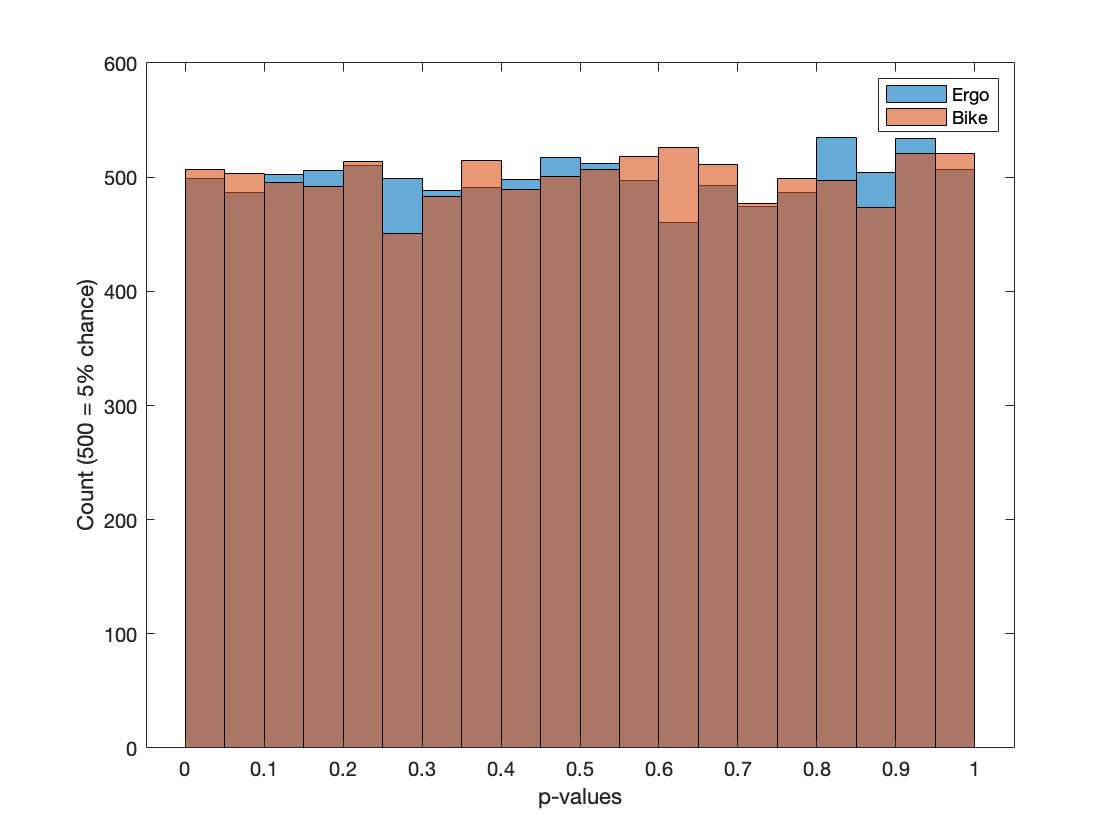
\includegraphics[width=\maxwidth{56.196688409433015em}]{figure_4.png}
\end{center}

\begin{par}
\begin{flushleft}
Test if p-value distribution is significantly different from a uniform distribution. h=0 confirms the null.
\end{flushleft}
\end{par}

\begin{matlabcode}
unipdf = makedist('uniform');
[hErgo,pErgo] = kstest(rhoErgo,'cdf',unipdf)
\end{matlabcode}
\begin{matlaboutput}
hErgo = 
   0

pErgo = 0.3280
\end{matlaboutput}
\begin{matlabcode}
[hBike,pBike] = kstest(rhoBike,'cdf',unipdf)
\end{matlabcode}
\begin{matlaboutput}
hBike = 
   0

pBike = 0.8356
\end{matlaboutput}


\begin{par}
\begin{flushleft}
As expected the p-value distribution is uniform (random). Now let's try a sample of 3 sprints.
\end{flushleft}
\end{par}

\begin{matlabcode}
nSamples = 3;
for i = 1:10000
    sample1 = random(pdErgo,nSamples,1);
    sample2 = random(pdErgo,nSamples,1);
    [~,p] = ttest2(sample1,sample2);
    rhoErgo(i) = p;
    sample1 = random(pdBike,nSamples,1);
    sample2 = random(pdBike,nSamples,1);
    [~,p] = ttest2(sample1,sample2);
    rhoBike(i) = p;
end
histogram(rhoErgo,20)
hold on
histogram(rhoBike,20)
hold off
xlabel('Count')
ylabel('p-values')
legend('Ergo','Bike')
\end{matlabcode}
\begin{center}
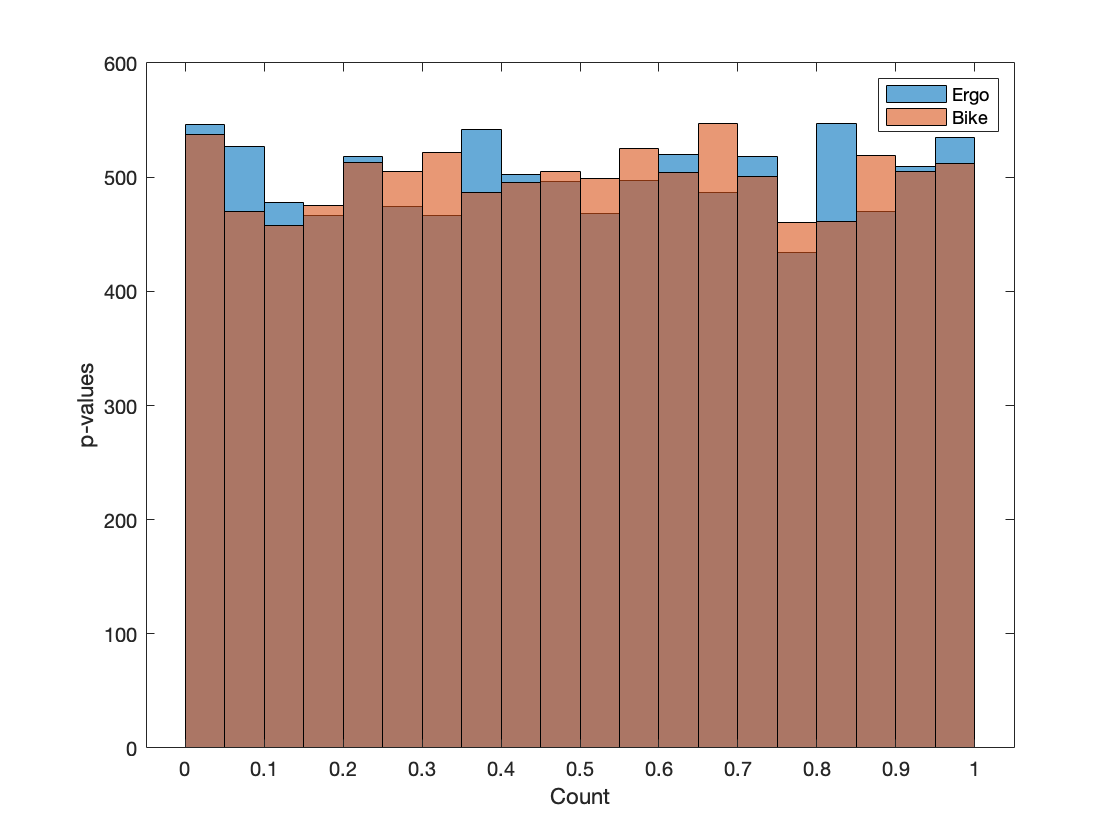
\includegraphics[width=\maxwidth{56.196688409433015em}]{figure_5.png}
\end{center}

\begin{par}
\begin{flushleft}
Test if p-value distribution is significantly different from a uniform distribution. h=0 confirms the null.
\end{flushleft}
\end{par}

\begin{matlabcode}
unipdf = makedist('uniform');
[hErgo,pErgo] = kstest(rhoErgo,'cdf',unipdf)
\end{matlabcode}
\begin{matlaboutput}
hErgo = 
   0

pErgo = 0.4285
\end{matlaboutput}
\begin{matlabcode}
[hBike,pBike] = kstest(rhoBike,'cdf',unipdf)
\end{matlabcode}
\begin{matlaboutput}
hBike = 
   0

pBike = 0.7662
\end{matlaboutput}

\begin{par}
\begin{flushleft}
It appears that getting subjects to perform 3 sprints will still provide an accurate estimation of their true mean.
\end{flushleft}
\end{par}


\matlabheading{Determine the uncertainty of the measurement and how it changes as we collect more sprints}

\begin{par}
\begin{flushleft}
If we assume that the mean over 12 sprints is our best estimate of the true mean, then we can calculate the root mean square error of each batch of measurements (i.e. n=1, n=2, etc.) relative to the mean. We want the uncertainty to be as low as possible, but does this uncertainty increase as we collect less and less measurements? 
\end{flushleft}
\end{par}

\begin{matlabcode}
y1rmseErgo = rms(meanPwrErgo - maxPowerErgo(1));
y2rmseErgo = rms(meanPwrErgo - maxPowerErgo(1:2));
y3rmseErgo = rms(meanPwrErgo - maxPowerErgo(1:3));
y4rmseErgo = rms(meanPwrErgo - maxPowerErgo(1:4));
y5rmseErgo = rms(meanPwrErgo - maxPowerErgo(1:5));
y6rmseErgo = rms(meanPwrErgo - maxPowerErgo(1:6));
y7rmseErgo = rms(meanPwrErgo - maxPowerErgo(1:7));
y8rmseErgo = rms(meanPwrErgo - maxPowerErgo(1:8));
y9rmseErgo = rms(meanPwrErgo - maxPowerErgo(1:9));
y10rmseErgo = rms(meanPwrErgo - maxPowerErgo(1:10));
y11rmseErgo = rms(meanPwrErgo - maxPowerErgo(1:11));
y12rmseErgo = rms(meanPwrErgo - maxPowerErgo(1:12));

yErgo = [y1rmseErgo/meanPwrErgo*100; y2rmseErgo/meanPwrErgo*100;...
    y3rmseErgo/meanPwrErgo*100; y4rmseErgo/meanPwrErgo*100;...
    y5rmseErgo/meanPwrErgo*100; y6rmseErgo/meanPwrErgo*100;...
    y7rmseErgo/meanPwrErgo*100; y8rmseErgo/meanPwrErgo*100;...
    y9rmseErgo/meanPwrErgo*100; y10rmseErgo/meanPwrErgo*100;...
    y11rmseErgo/meanPwrErgo*100; y12rmseErgo/meanPwrErgo*100];

y1rmseBike = rms(meanPwrBike - maxPowerBike(1));
y2rmseBike = rms(meanPwrBike - maxPowerBike(1:2));
y3rmseBike = rms(meanPwrBike - maxPowerBike(1:3));
y4rmseBike = rms(meanPwrBike - maxPowerBike(1:4));
y5rmseBike = rms(meanPwrBike - maxPowerBike(1:5));
y6rmseBike = rms(meanPwrBike - maxPowerBike(1:6));
y7rmseBike = rms(meanPwrBike - maxPowerBike(1:7));
y8rmseBike = rms(meanPwrBike - maxPowerBike(1:8));
y9rmseBike = rms(meanPwrBike - maxPowerBike(1:9));
y10rmseBike = rms(meanPwrBike - maxPowerBike(1:10));
y11rmseBike = rms(meanPwrBike - maxPowerBike(1:11));
y12rmseBike = rms(meanPwrBike - maxPowerBike(1:12));

yBike = [y1rmseBike/meanPwrBike*100; y2rmseBike/meanPwrBike*100;...
    y3rmseBike/meanPwrBike*100; y4rmseBike/meanPwrBike*100;...
    y5rmseBike/meanPwrBike*100; y6rmseBike/meanPwrBike*100;...
    y7rmseBike/meanPwrBike*100; y8rmseBike/meanPwrBike*100;...
    y9rmseBike/meanPwrBike*100; y10rmseBike/meanPwrBike*100;...
    y11rmseBike/meanPwrBike*100; y12rmseBike/meanPwrBike*100];

plot(yErgo,'o-')
hold on
plot(yBike,'o-')
hold off
legend('Ergo','Bike')
xlabel('Number of trials')
ylabel('Relative uncertainty of the measurement (%)')
ylim([0 3])
\end{matlabcode}
\begin{center}
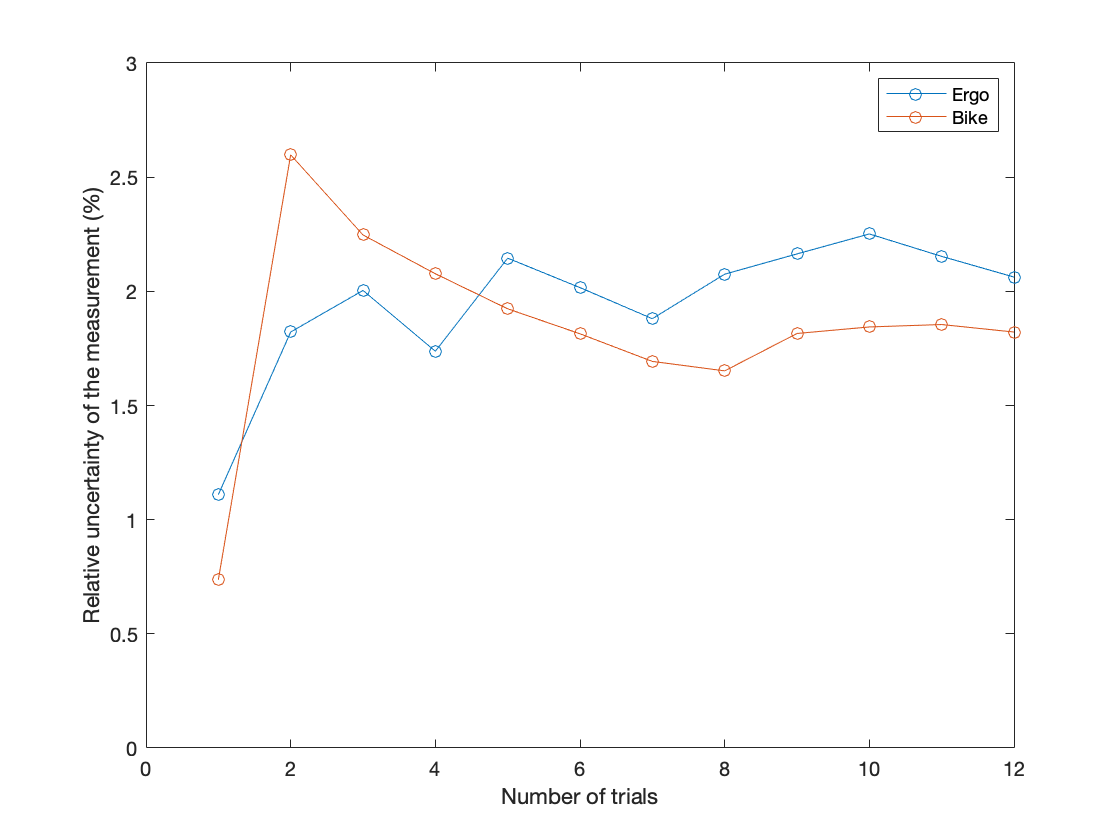
\includegraphics[width=\maxwidth{56.196688409433015em}]{figure_6.png}
\end{center}

\begin{par}
\begin{flushleft}
The uncertainty appears to be quite stable between 1.5-2.5\% from 3 sprints onwards during both ergometer and outdoor sprints. 
\end{flushleft}
\end{par}

\end{document}
